\documentclass[12pt]{article}
\usepackage{fullpage,enumitem,amsmath,amssymb,graphicx}
\usepackage{graphicx} % This is a package for including graphics in your solution.
\usepackage{listings}
\usepackage[final]{pdfpages}

\begin{document}

\begin{center}
{\Large CS168 Spring Assignment 8}

\begin{tabular}{rl}
SUNet ID(s): 05794739 & \\
Name(s): & Luis A. Perez \\
Collaborators: &
\end{tabular}
\end{center}

By turning in this assignment, I agree by the Stanford honor code and declare
that all of this is my own work.

\section*{Part 1}

\begin{enumerate}[label=(\alph*)]
  \item
    \begin{enumerate}
      \item Figure 1 on the LHS maps to Figure 5 on the RHS. Multiplying the fourier matrix $M$ by $1$ just means we sum elements in each row. For all rows except the first, the summation cancels out. 
      \item Figure 2 on the LHS maps to Figure 4 on the RHS. Multiplying the fourier matrix $M$ by the unit vector simply extract the corresponding column.
      \item Figure 3 on the LHS maps to Figure 1 on the RHS. This is becausee we're summing multiple columns of our fourier matrix, and the first and last column nearly cancel out.
      \item Fugure 4 on the LHS maps to Figure 7 on the RHS. This is because the figure is composed of just one frequent wave that goes from -1, 1, -1, 1, -1, ... and so on.
      \item Figure 5 on the LHS maps to Figure 3 on the RHS. This is because it's simply the sum of all of our frequencies, which lead to a stair-case pattern.
      \item Figure 6 on the LHS maps to Figure 6 on the RHS. This is because the fourier transform of a gaussian is a gausian.
      \item Figure 7 on the LHS maps to Figure 2 on the RHS. The distribution of elements is fairly complex, so it must consists of a combination of many different frequencies.
    \end{enumerate}
\end{enumerate}

\newpage
\section*{Part 2}

\begin{enumerate}[label=(\alph*)]
  \item This corresponds to the probability of the event that we after rolling a six-sided die 100 times, the sum of the results is equal to precisely $250$. 

  We can derive this directly. Consider simply the case $p * p$. In this situation, after convolving, we end with a vector of size $11$. The first entry simply corresponds to the probability of rollowing two $1$s. The second entry to the probability of rolling either a $1,2$ or a $2,1$. The third entry to the probability of rollowing a $1,3$, $3,1$, or $2,2$ (sum to 4). More generally, the $i$-th entry corresponds to the coefficient of $x^i$, which corresponds to the probability of rolling 2 numbers such that they sum to $i + 2$.

  Repeating this proceess $n$ times means that the $i$-th entry of the resulting vector corresponds to the coefficient of the $x^i$ term which corresponds to the probability of rolling $n$ numbers such that they sum to $i + n$.

  \item Consider the $k$-th index. We show that they are equivalent for the LHS and RHS. Let us being with the LHS. We have:
  \begin{align*}
    \mathcal{F}(\textbf{f} * \textbf{g})[k] &= \sum_{j=0}^{2N-1} (\textbf{f} * \textbf{g})[j]e^{-\frac{\pi i}{N}kj} \tag{Definition of discrete fourier transform} \\
    &= \sum_{j=0}^{2N - 1} \sum_{m=0}^{N-1} \textbf{f}[m]\textbf{g}[j - m]e^{-\frac{\pi i}{N}kj}
  \end{align*}
  For the RHS, we have:
  \begin{align*}
    (\mathcal{F}\textbf{f}^{+} \cdot \mathcal{F}\textbf{g}^{+})[k] &= \left( \sum_{j=0}^{2N - 1} \textbf{f}^{+}[j]e^{- \frac{\pi i}{N} kj} \right) \cdot \left( \sum_{j=0}^{2N-1} \textbf{g}^{+}[j]e^{- \frac{\pi i}{N} kj} \right) \\
    &= \left( \sum_{j=0}^{N - 1} \textbf{f}[j]e^{- \frac{\pi i}{N} kj} \right) \cdot \left( \sum_{j=0}^{N-1} \textbf{g}[j]e^{- \frac{\pi i}{N} kj} \right) \tag{Definition of $^{+}$} \\
    &= \sum_{m=0}^{2N - 1} \sum_{j=0}^{N-1} \textbf{f}[j]\textbf{g}[m - j]e^{-\frac{\pi i}{N}kj} \tag{Definition of multiplication}
  \end{align*}

  The above verifes that the LHS is equal to the RHS. With this confirmation, we can implement a convolution by taking the inverse fourier transform of both sides. We'll have:
  \[
    \textbf{f} * \textbf{g} = \mathcal{F}^{-1}(F \textbf{f}^{+} \cdot \mathcal{F}\textbf{g}^{+})
  \]
  If the two tuples have different lengths, since the convolution operation is translation invariant, we can simply shift the smaller vector (WLOG, assume this to be $\textbf{f}$) such that it is the same length as the larger vector. Then we can apply the same approach as before.

  \item
    We use the following code:
    \begin{verbatim}
from scipy import fft

def convolve(x: List[int], y:List[int]):
    """Compute x*y.
    
    Only accepts real-valued x,y.
    """
    m, l = len(x), len(y)
    n = max(m, l)
    x = x + [0] * (n + max(n - m, 0))
    y = y + [0] * (n + max(n - l, 0))
    assert len(x) == 2*n
    assert len(y) == 2*n
    return np.rint(np.real(fft.ifft(fft.fft(x) * fft.fft(y))[:m + l - 1])).astype(int)
    

def multiply(x: List[int], y: List[int]):
    """Multiplies x and y.
    
    Args:
        x: A list of digits. Lower indeces represent lower digits.
        y: Same as ax.
        
    Returns:
        A list of the same format representing the product x*y.
    """
    # Convolve the two using FFT.
    product = convolve(x, y)
    # Limit values to just be single digit.
    carry = 0
    fixed_product = []
    for val in product:
        digit = (val + carry) % 10
        carry = (val + carry) // 10
        fixed_product.append(int(np.rint(digit)))
        
    while carry > 0:
        digit = carry % 10
        carry = carry // 10
        fixed_product.append(int(np.rint(digit)))
    return fixed_product

def to_list(x: str) -> List[int]:
    return [int(char) for char in reversed(x)]

def from_list(x: List[int]) -> str:
    return "".join([str(y) for y in reversed(x)])

def problem2c():
    x = "12345678901234567890"
    y = "987654321098765432109876543210"
    print(f"{x} x {y} = {from_list(multiply(to_list(x), to_list(y)))}")
    \end{verbatim}

    We have the following results:

    12345678901234567890 x 987654321098765432109876543210 = 12193263113702179522496570642237463801111263526900

  \item
    The naive grade-school multiplication algorithm takes $O(n^2)$ time while the algorithm used above takes only $O(n \log n)$ time since the most expensive operation is the fast fourier transform (and its inverse). The element-wise product and processing are all linear time.

  \item
    TODO.
\end{enumerate}


\newpage
\section*{Part 2}

\begin{enumerate}[label=(\alph*)]
  \item
    I hear ``Laurel''.
  \item The requested plot is available in Figure \ref{fig:laurel_yanny_waveform}.
    \begin{figure}[!ht]
      \centering
      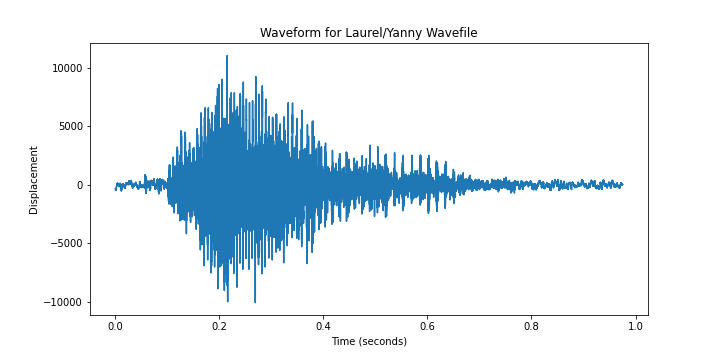
\includegraphics[scale=0.5]{figures/laurel_yanny_waveform.png}
      \caption{Laurel/Yanny Audio Waveform over Time}
      \label{fig:laurel_yanny_waveform}
    \end{figure}

  \item
    The requested plot is available in Figure \ref{fig:laurel_yanny_waveform_fft}. We see that this plot has two mode -- one around the low frequency range and one along the high frequency range. This is expected because these frequencies are just opposite of each other (inverse relation), so we they both correspond to the human audiable range.
    \begin{figure}[!ht]
      \centering
      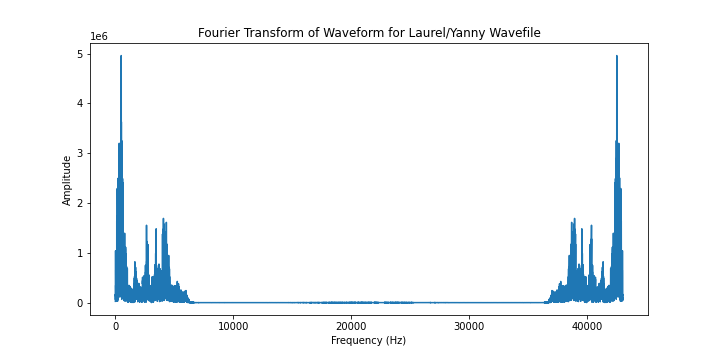
\includegraphics[scale=0.5]{figures/laurel_yanny_waveform_fft.png}
      \caption{Fourier Transform of Laurel/Yanny Audio Waveform}
      \label{fig:laurel_yanny_waveform_fft}
    \end{figure}

  \item The requested spectogram is available in Figure \ref{fig:spectogram}.
    \begin{figure}[!ht]
      \centering
      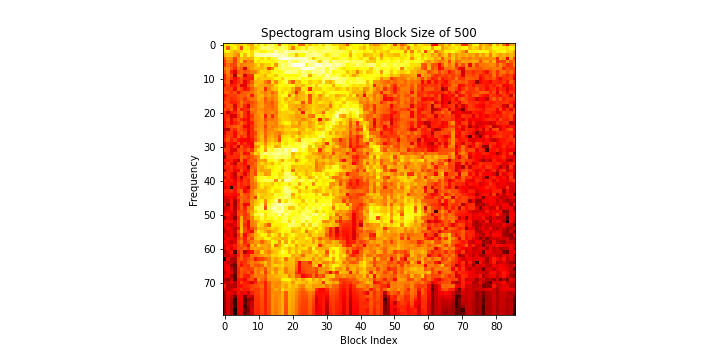
\includegraphics[scale=0.8]{figures/spectogram.png}
      \caption{Laurel/Yanny Audio Spectogram}
      \label{fig:spectogram}
    \end{figure}
  \item
    We took the approach of zeroing out the low and high frequencies (on both ends of the polynomial, after performing a FFT). However, no matter the thresholds we explored, we always heard ``Laurel'' in both versions.

  \item
    It was difficult to hear a difference, but it appears that for the more slowed down versions (factors in 0.25 and 0.5), a clear initial $y$ sounds was introduced into the audio.

\end{enumerate}




\newpage
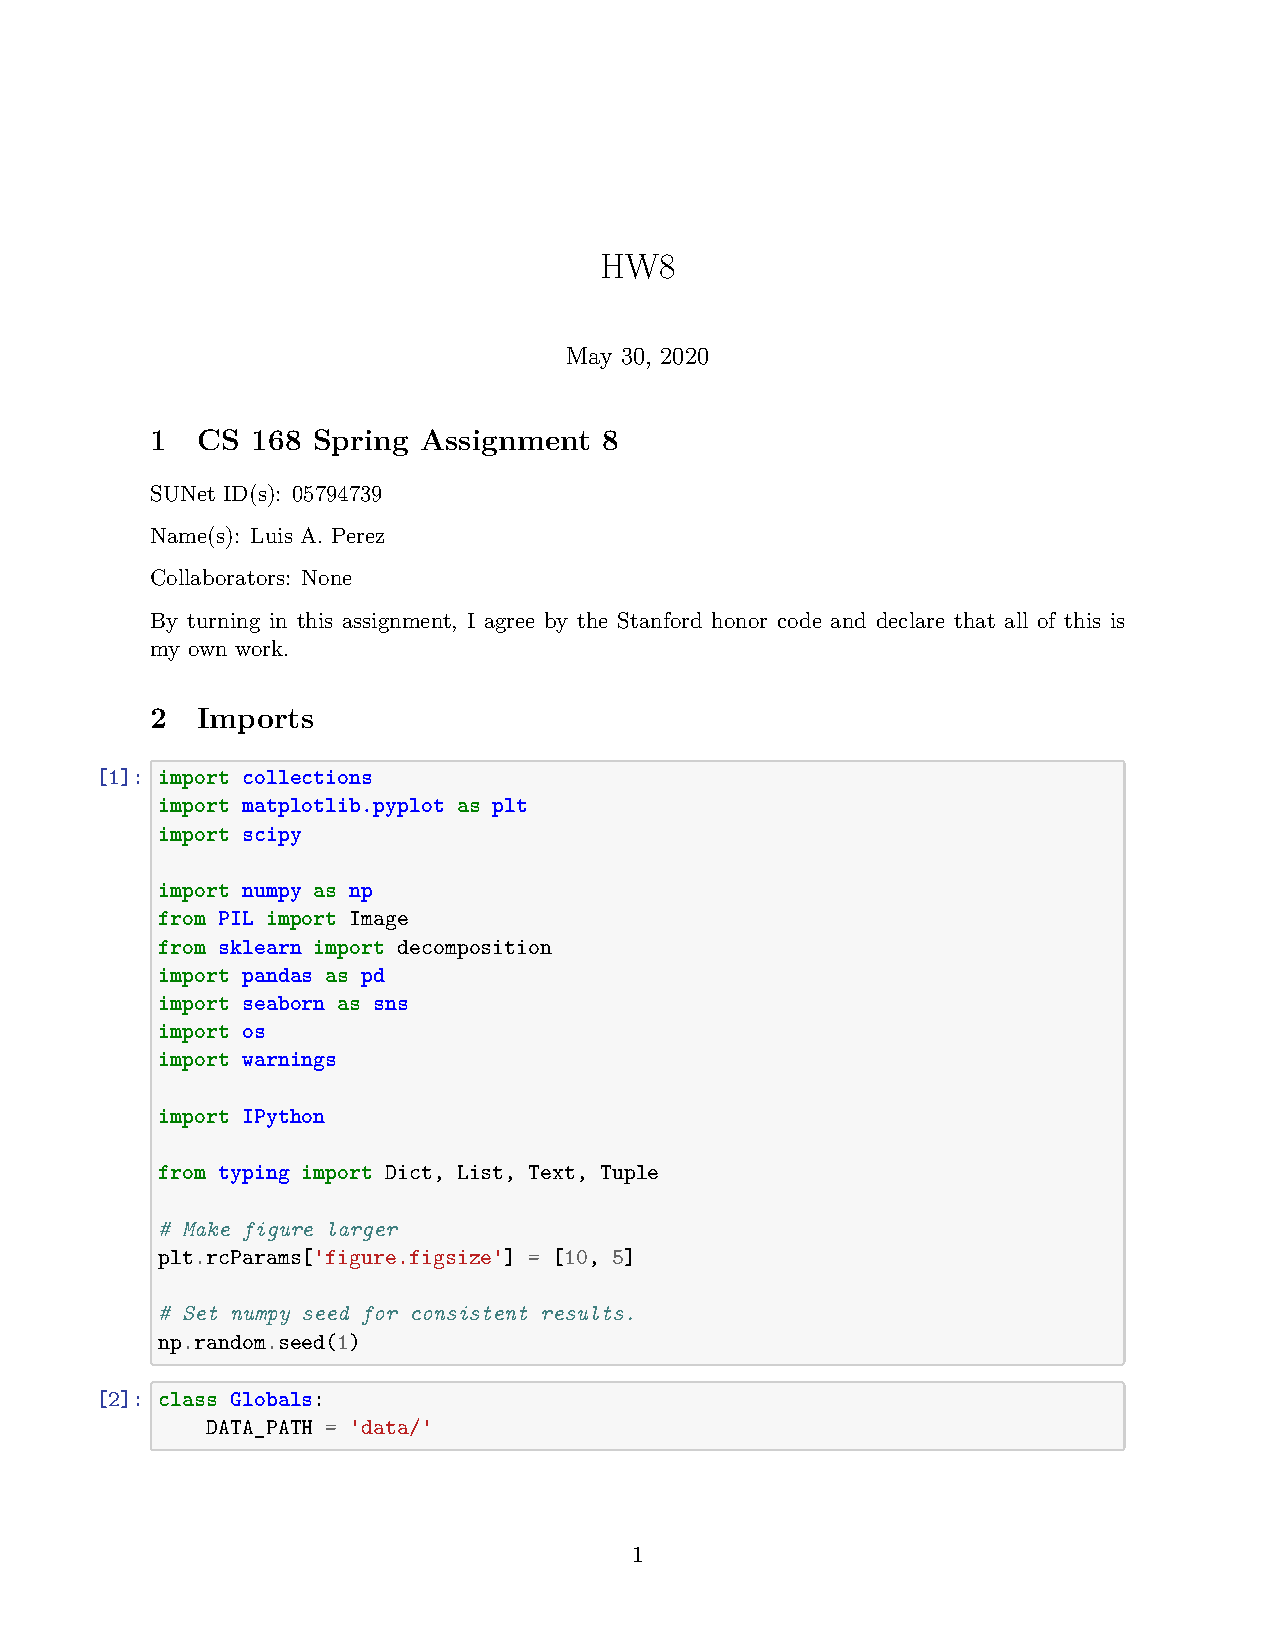
\includepdf[pages=-]{HW8}












\end{document}
